% ============================================================
% Question Bank: ch01-01 Unit Rates with Fractions
% Topic Title: Unit Rates with Fractions
% CCSS: 7.RP.A.1
% Questions: 30 (18 MC + 7 SA + 5 Graphical)
% ============================================================

% --- Multiple Choice Questions (18) ---

\begin{practiceQuestion}{1-1-q01}{mc}
\begin{questionText}
A recipe uses $\frac{3}{4}$ cup of flour for $\frac{1}{2}$ batch. How many cups of flour are needed per batch?
\end{questionText}
\choiceA{$\frac{3}{8}$}
\choiceB{$1\frac{1}{4}$}
\choiceC{$1\frac{1}{2}$}
\choiceD{$\frac{2}{3}$}
\correctAnswer{C}
\explanation{$\frac{3}{4} \div \frac{1}{2} = \frac{3}{4} \times \frac{2}{1} = \frac{6}{4} = \frac{3}{2} = 1\frac{1}{2}$ cups per batch.}
\end{practiceQuestion}

\begin{practiceQuestion}{1-1-q02}{mc}
\begin{questionText}
A hiker walks $\frac{2}{3}$ mile in $\frac{1}{4}$ hour. What is the hiker's speed in miles per hour?
\end{questionText}
\choiceA{$\frac{1}{6}$ mph}
\choiceB{$\frac{8}{12}$ mph}
\choiceC{$2\frac{2}{3}$ mph}
\choiceD{$3$ mph}
\correctAnswer{C}
\explanation{$\frac{2}{3} \div \frac{1}{4} = \frac{2}{3} \times \frac{4}{1} = \frac{8}{3} = 2\frac{2}{3}$ mph.}
\end{practiceQuestion}

\begin{practiceQuestion}{1-1-q03}{mc}
\begin{questionText}
A machine fills $\frac{5}{6}$ of a tank in $\frac{2}{3}$ hour. How many tanks does it fill per hour?
\end{questionText}
\choiceA{$\frac{5}{9}$}
\choiceB{$1\frac{1}{4}$}
\choiceC{$\frac{10}{9}$}
\choiceD{$2$}
\correctAnswer{B}
\explanation{$\frac{5}{6} \div \frac{2}{3} = \frac{5}{6} \times \frac{3}{2} = \frac{15}{12} = \frac{5}{4} = 1\frac{1}{4}$ tanks per hour.}
\end{practiceQuestion}

\begin{practiceQuestion}{1-1-q04}{mc}
\begin{questionText}
Lisa paints $\frac{1}{3}$ of a fence in $\frac{1}{2}$ hour. At this rate, how much of the fence can she paint in one hour?
\end{questionText}
\choiceA{$\frac{1}{6}$}
\choiceB{$\frac{1}{3}$}
\choiceC{$\frac{2}{3}$}
\choiceD{$1$}
\correctAnswer{C}
\explanation{$\frac{1}{3} \div \frac{1}{2} = \frac{1}{3} \times \frac{2}{1} = \frac{2}{3}$ of the fence per hour.}
\end{practiceQuestion}

\begin{practiceQuestion}{1-1-q05}{mc}
\begin{questionText}
A faucet drips $\frac{3}{8}$ cup of water in $\frac{3}{4}$ minute. What is the drip rate in cups per minute?
\end{questionText}
\choiceA{$\frac{9}{32}$}
\choiceB{$\frac{1}{2}$}
\choiceC{$\frac{3}{4}$}
\choiceD{$2$}
\correctAnswer{B}
\explanation{$\frac{3}{8} \div \frac{3}{4} = \frac{3}{8} \times \frac{4}{3} = \frac{12}{24} = \frac{1}{2}$ cup per minute.}
\end{practiceQuestion}

\begin{practiceQuestion}{1-1-q06}{mc}
\begin{questionText}
To find a unit rate when both quantities are fractions, you should:
\end{questionText}
\choiceA{Multiply the two fractions}
\choiceB{Add the two fractions}
\choiceC{Divide the first quantity by the second quantity}
\choiceD{Subtract the second quantity from the first}
\correctAnswer{C}
\explanation{A unit rate is found by dividing the first quantity by the second quantity to get the amount per one unit.}
\end{practiceQuestion}

\begin{practiceQuestion}{1-1-q07}{mc}
\begin{questionText}
A car uses $\frac{5}{6}$ gallon of gas to travel $\frac{2}{3}$ mile. How many gallons does it use per mile?
\end{questionText}
\choiceA{$\frac{5}{9}$}
\choiceB{$\frac{4}{5}$}
\choiceC{$1\frac{1}{4}$}
\choiceD{$1\frac{1}{2}$}
\correctAnswer{C}
\explanation{$\frac{5}{6} \div \frac{2}{3} = \frac{5}{6} \times \frac{3}{2} = \frac{15}{12} = \frac{5}{4} = 1\frac{1}{4}$ gallons per mile.}
\end{practiceQuestion}

\begin{practiceQuestion}{1-1-q08}{mc}
\begin{questionText}
Which expression shows the unit rate for $\frac{7}{8}$ pound per $\frac{1}{4}$ hour?
\end{questionText}
\choiceA{$\frac{7}{8} \times \frac{1}{4}$}
\choiceB{$\frac{7}{8} \div \frac{1}{4}$}
\choiceC{$\frac{1}{4} \div \frac{7}{8}$}
\choiceD{$\frac{7}{8} + \frac{1}{4}$}
\correctAnswer{B}
\explanation{The unit rate is found by dividing the first quantity by the second: $\frac{7}{8} \div \frac{1}{4} = \frac{7}{8} \times 4 = \frac{7}{2} = 3\frac{1}{2}$ pounds per hour.}
\end{practiceQuestion}

\begin{practiceQuestion}{1-1-q09}{mc}
\begin{questionText}
A garden hose fills $\frac{2}{5}$ of a pool in $\frac{4}{5}$ hour. What fraction of the pool is filled per hour?
\end{questionText}
\choiceA{$\frac{8}{25}$}
\choiceB{$\frac{1}{2}$}
\choiceC{$2$}
\choiceD{$\frac{2}{5}$}
\correctAnswer{B}
\explanation{$\frac{2}{5} \div \frac{4}{5} = \frac{2}{5} \times \frac{5}{4} = \frac{10}{20} = \frac{1}{2}$ pool per hour.}
\end{practiceQuestion}

\begin{practiceQuestion}{1-1-q10}{mc}
\begin{questionText}
A snail moves $\frac{5}{8}$ meter in $\frac{3}{4}$ hour. A beetle moves $\frac{7}{10}$ meter in $\frac{4}{5}$ hour. Which is faster?
\end{questionText}
\choiceA{The snail, at $\frac{5}{6}$ m/hr}
\choiceB{The beetle, at $\frac{7}{8}$ m/hr}
\choiceC{They are the same speed}
\choiceD{The snail, at $\frac{7}{8}$ m/hr}
\correctAnswer{B}
\explanation{Snail: $\frac{5}{8} \div \frac{3}{4} = \frac{5}{6}$ m/hr. Beetle: $\frac{7}{10} \div \frac{4}{5} = \frac{7}{8}$ m/hr. Since $\frac{7}{8} > \frac{5}{6}$, the beetle is faster.}
\end{practiceQuestion}

\begin{practiceQuestion}{1-1-q11}{mc}
\begin{questionText}
Sam reads $\frac{3}{4}$ of a chapter in $\frac{2}{3}$ hour. How many chapters does Sam read per hour?
\end{questionText}
\choiceA{$\frac{1}{2}$}
\choiceB{$\frac{8}{9}$}
\choiceC{$1\frac{1}{8}$}
\choiceD{$2$}
\correctAnswer{C}
\explanation{$\frac{3}{4} \div \frac{2}{3} = \frac{3}{4} \times \frac{3}{2} = \frac{9}{8} = 1\frac{1}{8}$ chapters per hour.}
\end{practiceQuestion}

\begin{practiceQuestion}{1-1-q12}{mc}
\begin{questionText}
A baker uses $\frac{2}{3}$ cup of sugar for every $\frac{1}{6}$ of a cake. How many cups of sugar are needed for a whole cake?
\end{questionText}
\choiceA{$\frac{1}{9}$}
\choiceB{$4$}
\choiceC{$3\frac{1}{2}$}
\choiceD{$\frac{2}{18}$}
\correctAnswer{B}
\explanation{$\frac{2}{3} \div \frac{1}{6} = \frac{2}{3} \times \frac{6}{1} = \frac{12}{3} = 4$ cups per cake.}
\end{practiceQuestion}

\begin{practiceQuestion}{1-1-q13}{mc}
\begin{questionText}
Which unit rate is the greatest?
\end{questionText}
\choiceA{$\frac{1}{2}$ mile in $\frac{1}{3}$ hour}
\choiceB{$\frac{3}{4}$ mile in $\frac{1}{2}$ hour}
\choiceC{$\frac{2}{5}$ mile in $\frac{1}{4}$ hour}
\choiceD{$\frac{1}{3}$ mile in $\frac{1}{5}$ hour}
\correctAnswer{D}
\explanation{A: $\frac{1}{2} \div \frac{1}{3} = \frac{3}{2} = 1.5$ mph. B: $\frac{3}{4} \div \frac{1}{2} = \frac{3}{2} = 1.5$ mph. C: $\frac{2}{5} \div \frac{1}{4} = \frac{8}{5} = 1.6$ mph. D: $\frac{1}{3} \div \frac{1}{5} = \frac{5}{3} \approx 1.67$ mph. D is the greatest.}
\end{practiceQuestion}

\begin{practiceQuestion}{1-1-q14}{mc}
\begin{questionText}
A pump moves $\frac{7}{10}$ liter of water in $\frac{1}{2}$ minute. How many liters does it move per minute?
\end{questionText}
\choiceA{$\frac{7}{20}$}
\choiceB{$\frac{7}{5}$}
\choiceC{$1$}
\choiceD{$2$}
\correctAnswer{B}
\explanation{$\frac{7}{10} \div \frac{1}{2} = \frac{7}{10} \times \frac{2}{1} = \frac{14}{10} = \frac{7}{5} = 1\frac{2}{5}$ liters per minute.}
\end{practiceQuestion}

\begin{practiceQuestion}{1-1-q15}{mc}
\begin{questionText}
Store A sells $\frac{3}{4}$ pound of cheese for $\$2$. Store B sells $\frac{1}{2}$ pound for $\$1.50$. Which store has the lower price per pound?
\end{questionText}
\choiceA{Store A at $\$2.67$ per pound}
\choiceB{Store B at $\$3.00$ per pound}
\choiceC{They are the same price per pound}
\choiceD{Store B at $\$2.50$ per pound}
\correctAnswer{A}
\explanation{Store A: $2 \div \frac{3}{4} = 2 \times \frac{4}{3} = \frac{8}{3} \approx \$2.67$/lb. Store B: $1.50 \div \frac{1}{2} = 1.50 \times 2 = \$3.00$/lb. Store A is cheaper.}
\end{practiceQuestion}

\begin{practiceQuestion}{1-1-q16}{mc}
\begin{questionText}
A runner completes $\frac{3}{5}$ of a lap in $\frac{2}{5}$ minute. How many laps does the runner complete per minute?
\end{questionText}
\choiceA{$\frac{6}{25}$}
\choiceB{$1\frac{1}{2}$}
\choiceC{$\frac{6}{5}$}
\choiceD{$2\frac{1}{2}$}
\correctAnswer{B}
\explanation{$\frac{3}{5} \div \frac{2}{5} = \frac{3}{5} \times \frac{5}{2} = \frac{15}{10} = \frac{3}{2} = 1\frac{1}{2}$ laps per minute.}
\end{practiceQuestion}

\begin{practiceQuestion}{1-1-q17}{mc}
\begin{questionText}
Maya jogs $\frac{4}{5}$ mile in $\frac{2}{3}$ hour. What is her speed in miles per hour?
\end{questionText}
\choiceA{$\frac{8}{15}$ mph}
\choiceB{$1\frac{1}{5}$ mph}
\choiceC{$1\frac{2}{3}$ mph}
\choiceD{$2$ mph}
\correctAnswer{B}
\explanation{$\frac{4}{5} \div \frac{2}{3} = \frac{4}{5} \times \frac{3}{2} = \frac{12}{10} = \frac{6}{5} = 1\frac{1}{5}$ mph.}
\end{practiceQuestion}

\begin{practiceQuestion}{1-1-q18}{mc}
\begin{questionText}
A factory produces $\frac{5}{6}$ of a toy in $\frac{5}{12}$ hour. How many toys does it produce per hour?
\end{questionText}
\choiceA{$\frac{25}{72}$}
\choiceB{$\frac{1}{2}$}
\choiceC{$2$}
\choiceD{$\frac{5}{7}$}
\correctAnswer{C}
\explanation{$\frac{5}{6} \div \frac{5}{12} = \frac{5}{6} \times \frac{12}{5} = \frac{60}{30} = 2$ toys per hour.}
\end{practiceQuestion}

% --- Short Answer Questions (7) ---

\begin{practiceQuestion}{1-1-q19}{sa}
\begin{questionText}
A pipe fills $\frac{3}{4}$ of a tank in $\frac{3}{8}$ hour. How many tanks does it fill per hour?
\end{questionText}
\correctAnswer{$2$}
\explanation{$\frac{3}{4} \div \frac{3}{8} = \frac{3}{4} \times \frac{8}{3} = \frac{24}{12} = 2$ tanks per hour.}
\end{practiceQuestion}

\begin{practiceQuestion}{1-1-q20}{sa}
\begin{questionText}
A cyclist rides $\frac{7}{8}$ mile in $\frac{1}{4}$ hour. What is the cyclist's speed in miles per hour?
\end{questionText}
\correctAnswer{$3\frac{1}{2}$ mph}
\explanation{$\frac{7}{8} \div \frac{1}{4} = \frac{7}{8} \times \frac{4}{1} = \frac{28}{8} = \frac{7}{2} = 3\frac{1}{2}$ mph.}
\end{practiceQuestion}

\begin{practiceQuestion}{1-1-q21}{sa}
\begin{questionText}
A printer uses $\frac{2}{5}$ of an ink cartridge to print $\frac{1}{3}$ of a book. How many cartridges does it use per book?
\end{questionText}
\correctAnswer{$1\frac{1}{5}$}
\explanation{$\frac{2}{5} \div \frac{1}{3} = \frac{2}{5} \times \frac{3}{1} = \frac{6}{5} = 1\frac{1}{5}$ cartridges per book.}
\end{practiceQuestion}

\begin{practiceQuestion}{1-1-q22}{sa}
\begin{questionText}
Trail A is $\frac{5}{6}$ mile long and takes $\frac{1}{3}$ hour to walk. What is the walking rate in miles per hour?
\end{questionText}
\correctAnswer{$2\frac{1}{2}$ mph}
\explanation{$\frac{5}{6} \div \frac{1}{3} = \frac{5}{6} \times \frac{3}{1} = \frac{15}{6} = \frac{5}{2} = 2\frac{1}{2}$ mph.}
\end{practiceQuestion}

\begin{practiceQuestion}{1-1-q23}{sa}
\begin{questionText}
A recipe calls for $\frac{5}{8}$ cup of oil per $\frac{1}{4}$ pan of brownies. How many cups of oil are needed for a full pan?
\end{questionText}
\correctAnswer{$2\frac{1}{2}$ cups}
\explanation{$\frac{5}{8} \div \frac{1}{4} = \frac{5}{8} \times \frac{4}{1} = \frac{20}{8} = \frac{5}{2} = 2\frac{1}{2}$ cups per pan.}
\end{practiceQuestion}

\begin{practiceQuestion}{1-1-q24}{sa}
\begin{questionText}
Worker A packs $\frac{3}{4}$ box in $\frac{1}{2}$ hour. Worker B packs $\frac{2}{3}$ box in $\frac{1}{3}$ hour. How many more boxes per hour does Worker B pack than Worker A?
\end{questionText}
\correctAnswer{$\frac{1}{2}$}
\explanation{Worker A: $\frac{3}{4} \div \frac{1}{2} = \frac{3}{2} = 1\frac{1}{2}$ boxes/hr. Worker B: $\frac{2}{3} \div \frac{1}{3} = 2$ boxes/hr. Difference: $2 - 1\frac{1}{2} = \frac{1}{2}$ box per hour.}
\end{practiceQuestion}

\begin{practiceQuestion}{1-1-q25}{sa}
\begin{questionText}
A truck uses $\frac{7}{8}$ gallon of fuel to travel $\frac{7}{16}$ mile. How many gallons of fuel does it use per mile?
\end{questionText}
\correctAnswer{$2$}
\explanation{$\frac{7}{8} \div \frac{7}{16} = \frac{7}{8} \times \frac{16}{7} = \frac{112}{56} = 2$ gallons per mile.}
\end{practiceQuestion}

% --- Graphical Questions (3 GMC + 2 GSA) ---

\begin{practiceQuestion}{1-1-q26}{gmc}
\begin{questionText}
The table below shows how much of a wall a painter covers in the given time. What is the unit rate in walls per hour?

\begin{center}
\begin{tabular}{|c|c|}
\hline
\textbf{Time (hr)} & \textbf{Wall covered} \\ \hline
$\frac{1}{4}$ & $\frac{1}{6}$ \\ \hline
$\frac{1}{2}$ & $\frac{1}{3}$ \\ \hline
$\frac{3}{4}$ & $\frac{1}{2}$ \\ \hline
\end{tabular}
\end{center}
\end{questionText}
\choiceA{$\frac{1}{24}$ wall per hour}
\choiceB{$\frac{1}{3}$ wall per hour}
\choiceC{$\frac{2}{3}$ wall per hour}
\choiceD{$1\frac{1}{2}$ walls per hour}
\correctAnswer{C}
\explanation{Divide any row: $\frac{1}{6} \div \frac{1}{4} = \frac{1}{6} \times 4 = \frac{4}{6} = \frac{2}{3}$ wall per hour.}
\end{practiceQuestion}

\begin{practiceQuestion}{1-1-q27}{gmc}
\begin{questionText}
Two runners start at the same time. The graph below shows the distance each has traveled. Who is faster?

\begin{center}
\begin{tikzpicture}[scale=0.9]
  \draw[step=1,gray!20,thin] (0,0) grid (5,5);
  \draw[thick,->] (0,0) -- (5.5,0) node[right]{\small Time (hr)};
  \draw[thick,->] (0,0) -- (0,5.5) node[above]{\small Distance (mi)};
  \foreach \x in {1,...,5} \draw (\x,0.07) -- (\x,-0.07) node[below]{\tiny \x};
  \foreach \y in {1,...,5} \draw (0.07,\y) -- (-0.07,\y) node[left]{\tiny \y};
  \draw[thick,funBlue] (0,0) -- (4,5);
  \fill[funBlue] (0,0) circle (2pt);
  \fill[funBlue] (4,5) circle (2pt) node[above left]{\small Runner A};
  \draw[thick,funRed] (0,0) -- (5,5);
  \fill[funRed] (0,0) circle (2pt);
  \fill[funRed] (5,5) circle (2pt) node[below right]{\small Runner B};
\end{tikzpicture}
\end{center}
\end{questionText}
\choiceA{Runner A, because the line is steeper}
\choiceB{Runner B, because the line is longer}
\choiceC{They are the same speed}
\choiceD{Cannot be determined from the graph}
\correctAnswer{A}
\explanation{Runner A's line is steeper, meaning a greater distance per unit of time. A steeper line on a proportional graph means a higher unit rate, so Runner A is faster.}
\end{practiceQuestion}

\begin{practiceQuestion}{1-1-q28}{gmc}
\begin{questionText}
The double number line below shows the relationship between cups of juice and servings. What is the unit rate in cups per serving?

\begin{center}
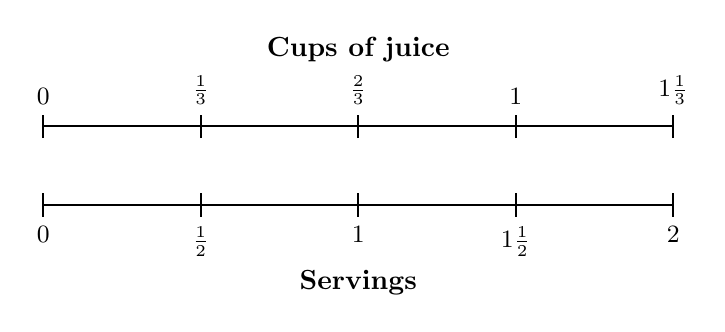
\begin{tikzpicture}[scale=1.0]
  % Top number line: cups
  \draw[thick] (0,1) -- (8,1);
  \foreach \x/\lab in {0/$0$, 2/$\frac{1}{3}$, 4/$\frac{2}{3}$, 6/$1$, 8/$1\frac{1}{3}$} {
    \draw[thick] (\x,0.85) -- (\x,1.15);
    \node[above] at (\x,1.15) {\small \lab};
  }
  \node[above] at (4,1.7) {\textbf{Cups of juice}};
  % Bottom number line: servings
  \draw[thick] (0,0) -- (8,0);
  \foreach \x/\lab in {0/$0$, 2/$\frac{1}{2}$, 4/$1$, 6/$1\frac{1}{2}$, 8/$2$} {
    \draw[thick] (\x,-0.15) -- (\x,0.15);
    \node[below] at (\x,-0.15) {\small \lab};
  }
  \node[below] at (4,-0.7) {\textbf{Servings}};
\end{tikzpicture}
\end{center}
\end{questionText}
\choiceA{$\frac{1}{3}$ cup per serving}
\choiceB{$\frac{1}{2}$ cup per serving}
\choiceC{$\frac{2}{3}$ cup per serving}
\choiceD{$1\frac{1}{2}$ cups per serving}
\correctAnswer{C}
\explanation{At 1 serving, the top number line reads $\frac{2}{3}$ cup. Or compute: $\frac{1}{3} \div \frac{1}{2} = \frac{1}{3} \times 2 = \frac{2}{3}$ cup per serving.}
\end{practiceQuestion}

\begin{practiceQuestion}{1-1-q29}{gsa}
\begin{questionText}
The table shows how much ribbon Maria uses for different numbers of gift bows. What is the unit rate in feet of ribbon per bow?

\begin{center}
\begin{tabular}{|c|c|}
\hline
\textbf{Bows} & \textbf{Ribbon (ft)} \\ \hline
$\frac{1}{3}$ & $\frac{5}{6}$ \\ \hline
$\frac{2}{3}$ & $\frac{5}{3}$ \\ \hline
$1$ & $\frac{5}{2}$ \\ \hline
\end{tabular}
\end{center}
\end{questionText}
\correctAnswer{$2\frac{1}{2}$ feet per bow}
\explanation{$\frac{5}{6} \div \frac{1}{3} = \frac{5}{6} \times 3 = \frac{15}{6} = \frac{5}{2} = 2\frac{1}{2}$ feet per bow. Confirmed by the third row: $\frac{5}{2} \div 1 = \frac{5}{2}$.}
\end{practiceQuestion}

\begin{practiceQuestion}{1-1-q30}{gsa}
\begin{questionText}
Two machines are filling containers. The table shows the fraction of a container each fills in the given time. Which machine is faster, and what is its rate in containers per hour?

\begin{center}
\begin{tabular}{|c|c|c|}
\hline
 & \textbf{Time (hr)} & \textbf{Containers filled} \\ \hline
Machine X & $\frac{2}{5}$ & $\frac{1}{2}$ \\ \hline
Machine Y & $\frac{1}{3}$ & $\frac{1}{4}$ \\ \hline
\end{tabular}
\end{center}
\end{questionText}
\correctAnswer{Machine X at $1\frac{1}{4}$ containers per hour}
\explanation{Machine X: $\frac{1}{2} \div \frac{2}{5} = \frac{1}{2} \times \frac{5}{2} = \frac{5}{4} = 1\frac{1}{4}$ containers/hr. Machine Y: $\frac{1}{4} \div \frac{1}{3} = \frac{1}{4} \times 3 = \frac{3}{4}$ containers/hr. Machine X is faster at $1\frac{1}{4}$ containers per hour.}
\end{practiceQuestion}
